\section{Results}
\begin{frame}{Experimental setup}
\begin{itemize}
  \item<1-> Experiments run on 3 platforms:
  \begin{itemize}
    \item \textbf{x86}: AMD EPYC 7543 CPU @ 2.8 GHz (32 cores)
    \item \textbf{RISC-V}: Sophon SG2042 CPU @ 2.0 GHz (64 cores)
    \item \textbf{ARM}: NVIDIA Grace CPU Superchip @ up to 3.0 GHz (144 cores)
  \end{itemize}
  \item<2-> Datasets: 3 road networks (USA, Europe, Asia), 3 FEM meshes (Earth's crust, steel hook, porous material), 1 random geometric graph (RGG)
  \item<3-> Tools: GCC compiler, SBatchMan
  \item<4-> Compared against the GAP benchmark suite \footfullcite{beamer2015gap}
\end{itemize}
\begin{figure}
  \centering
  
\includegraphics[height=1.4cm]{images/tools.png}
\end{figure}
\vspace{2mm}
\end{frame}

\begin{frame}{Scalability}
\begin{figure}
  \centering
  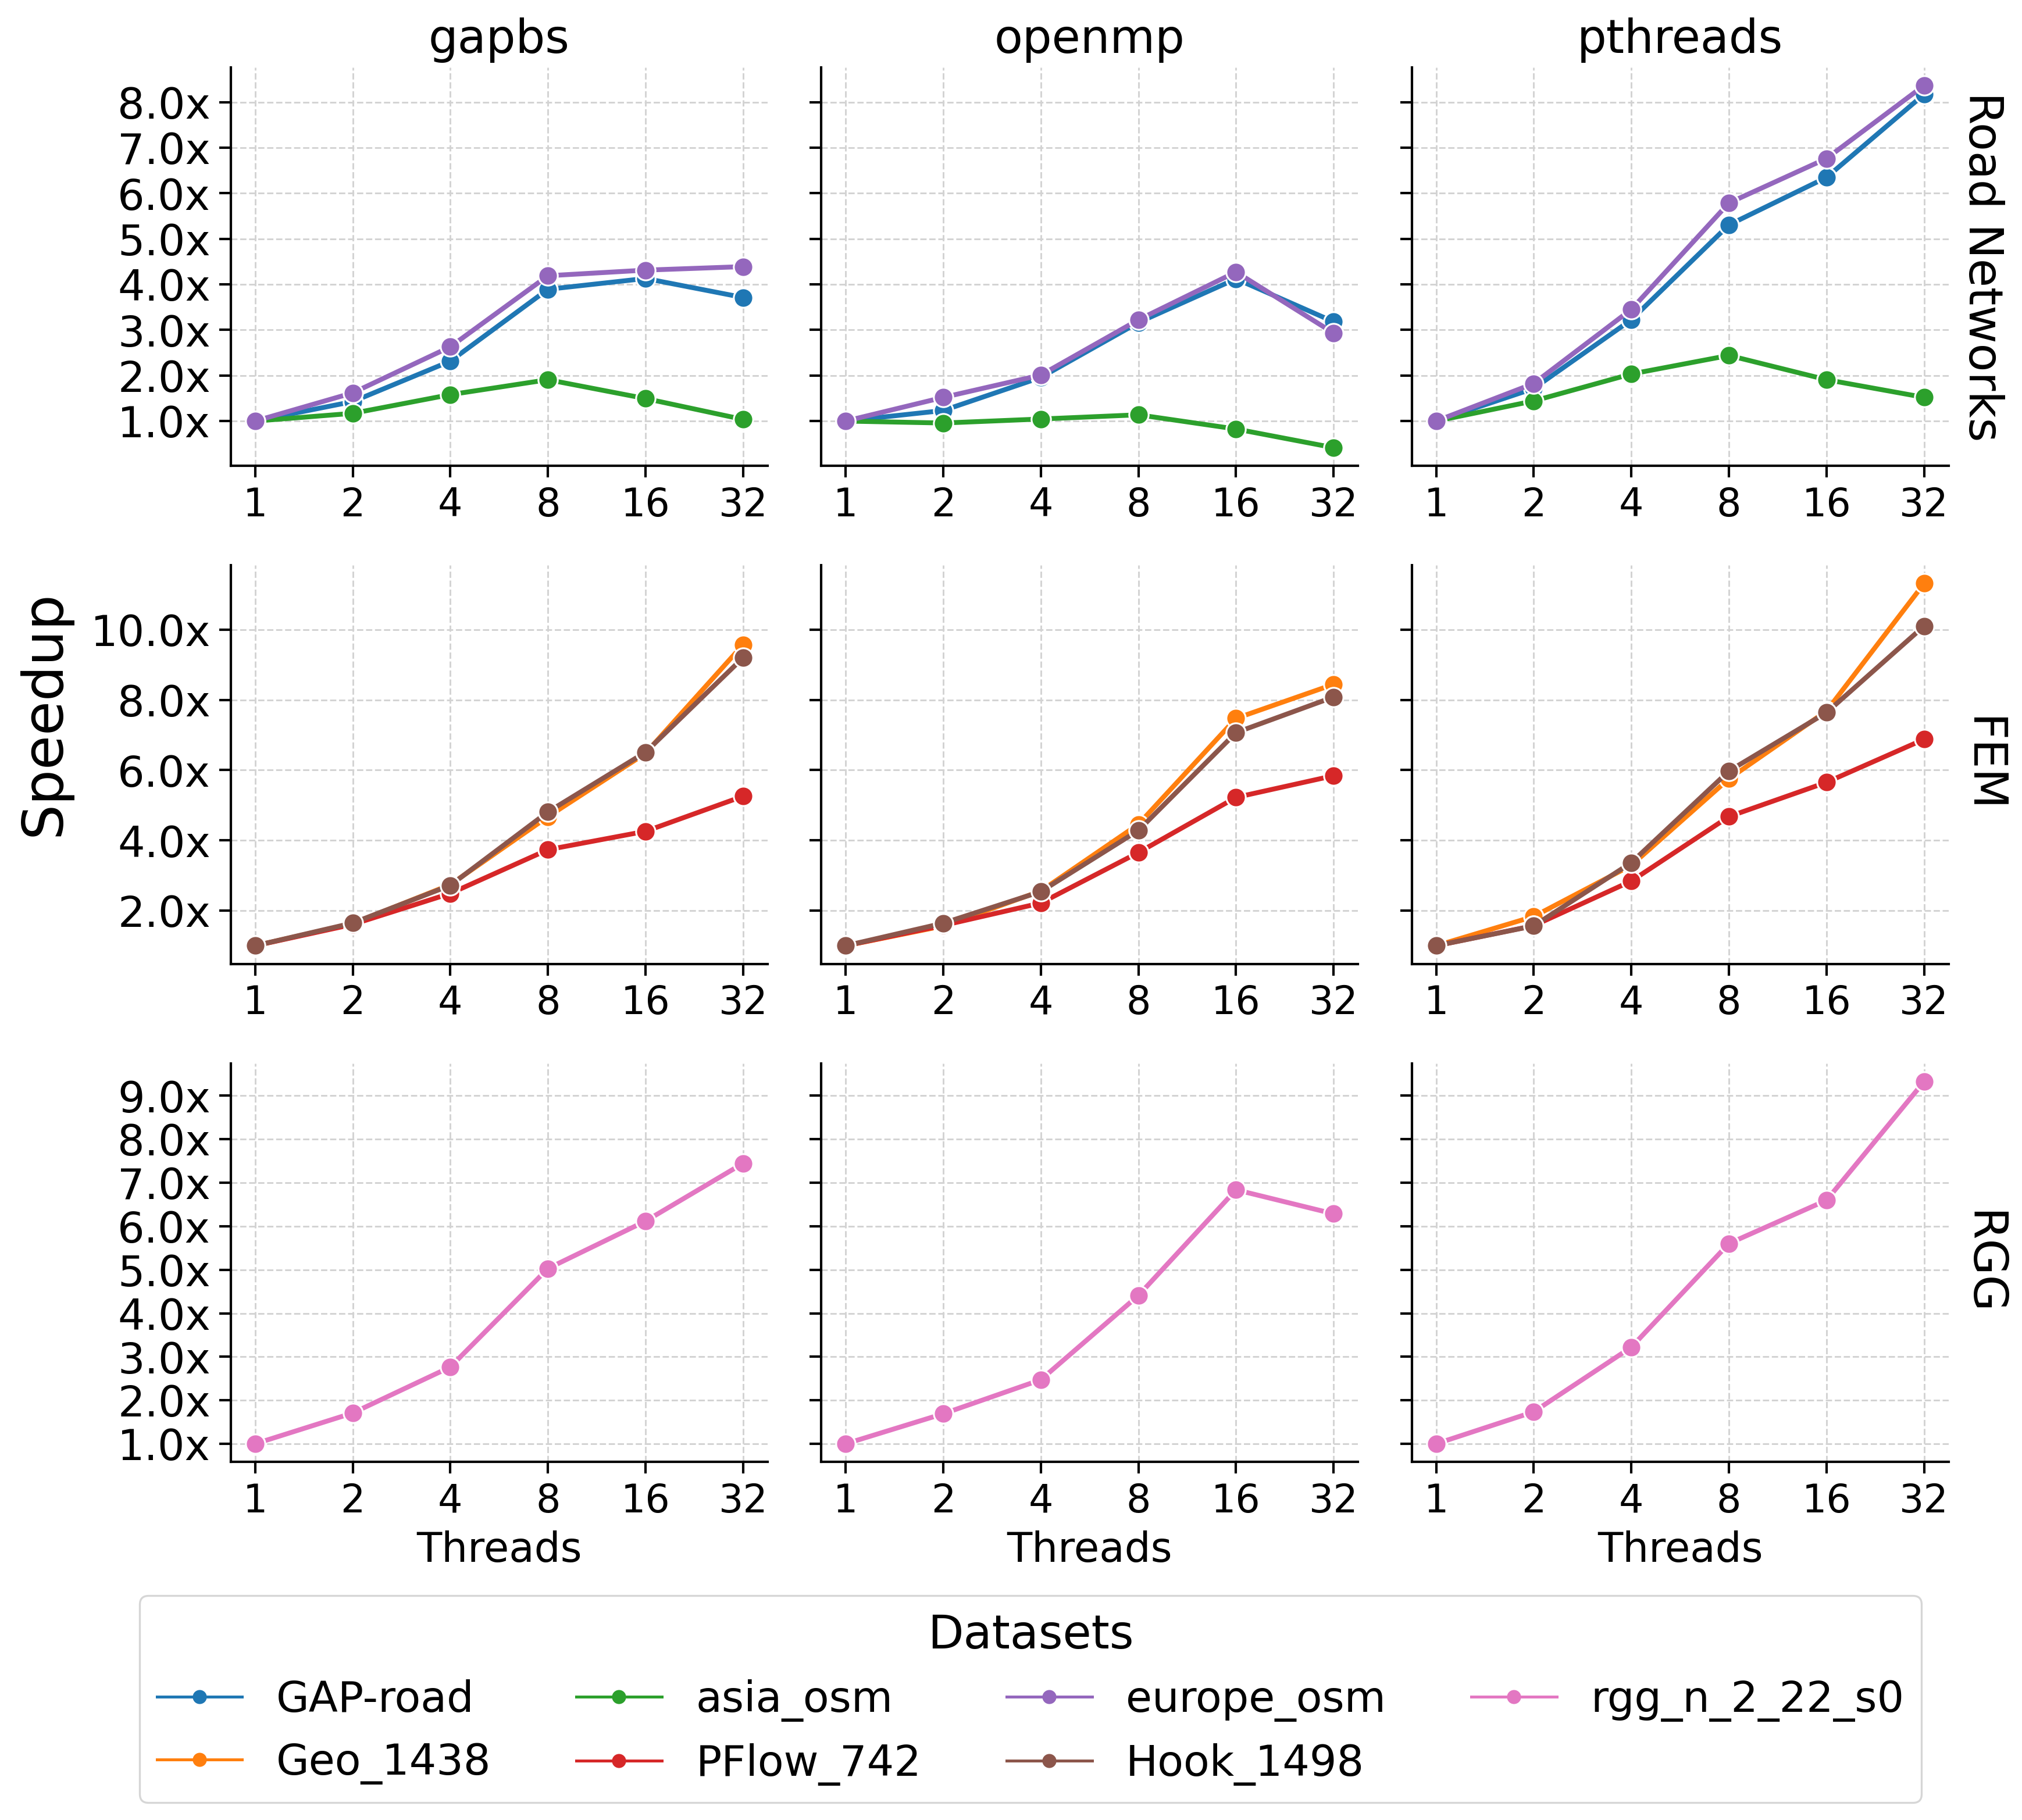
\includegraphics[width=0.6\linewidth]{images/scalability.png}
\end{figure}
\end{frame}

\begin{frame}{Speedup}
\begin{figure}
  \centering
  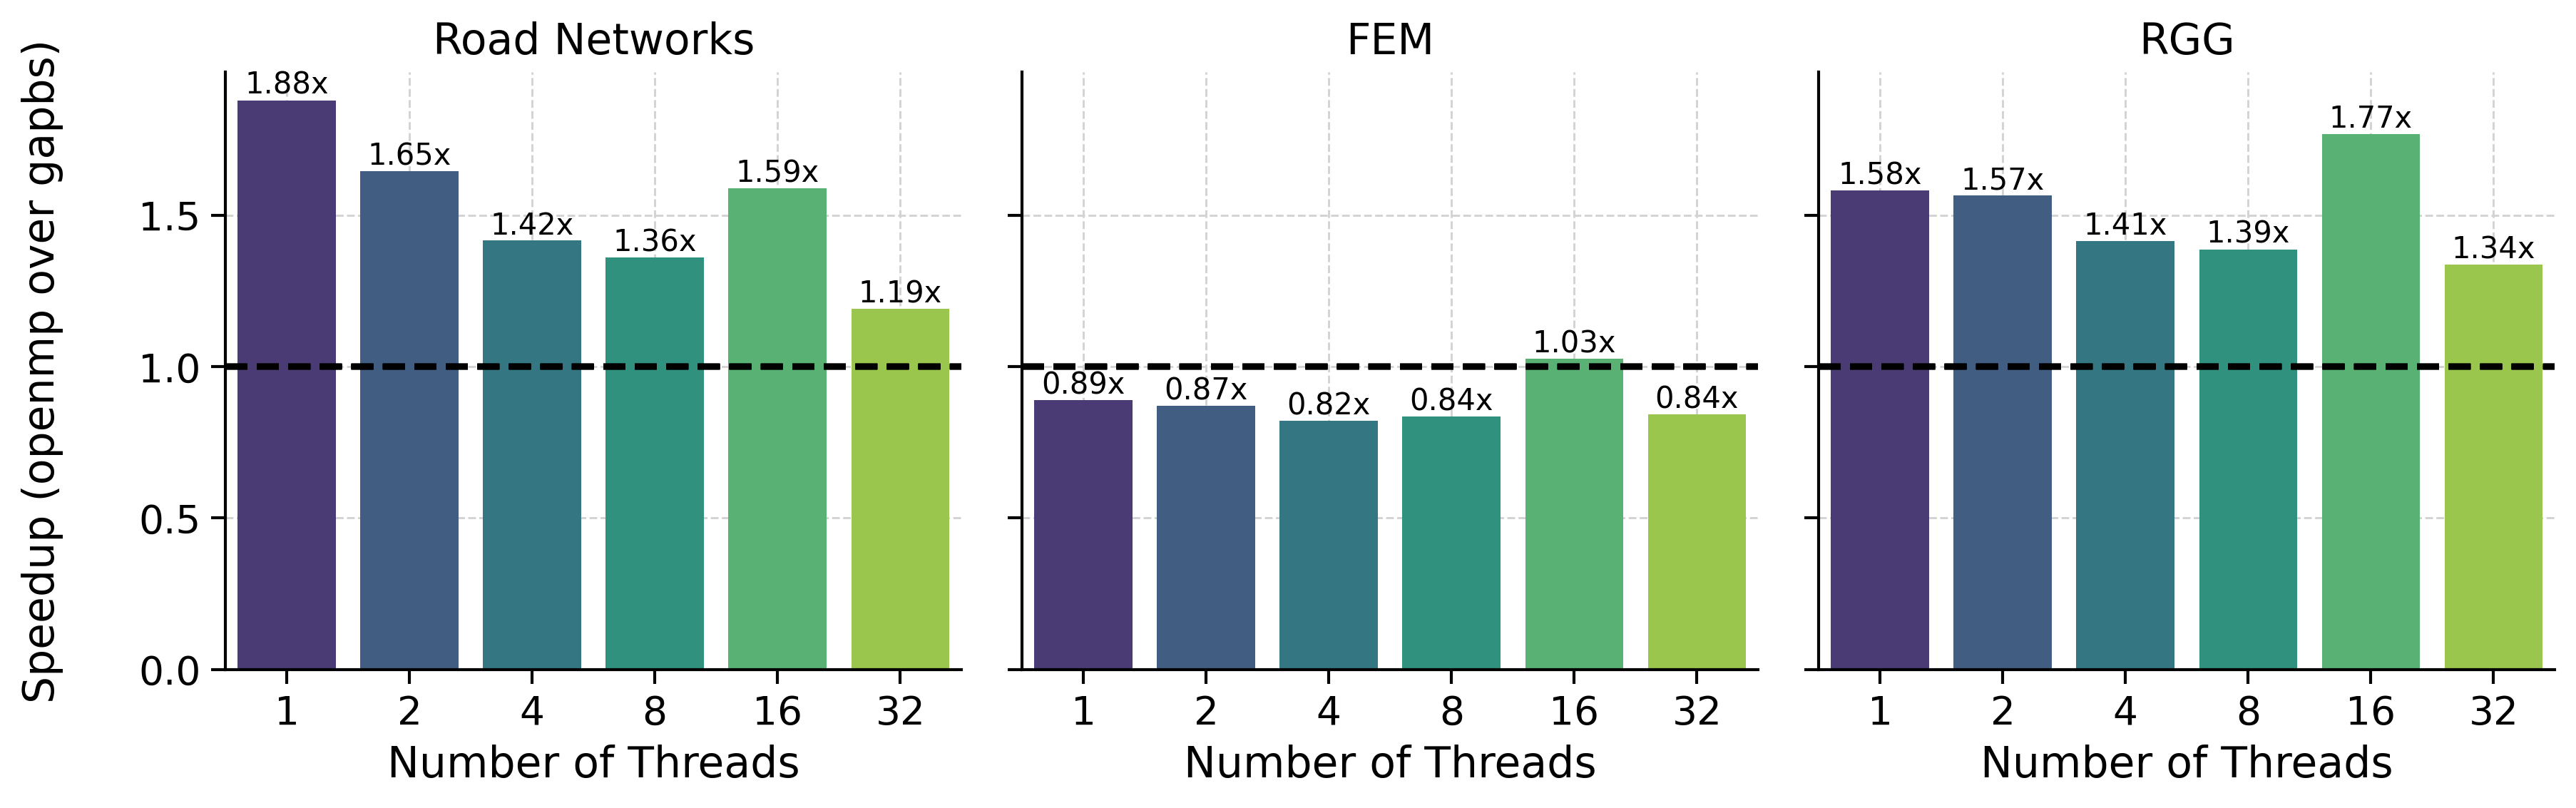
\includegraphics[width=0.7\linewidth]{images/speedup_openmp.png}
  \vspace{-2mm}
  \caption{\footnotesize Speedup of the OpenMP implementation compared to the GAPBS implementation}
\end{figure}
\vspace{-5mm}
\begin{figure}
  \centering
  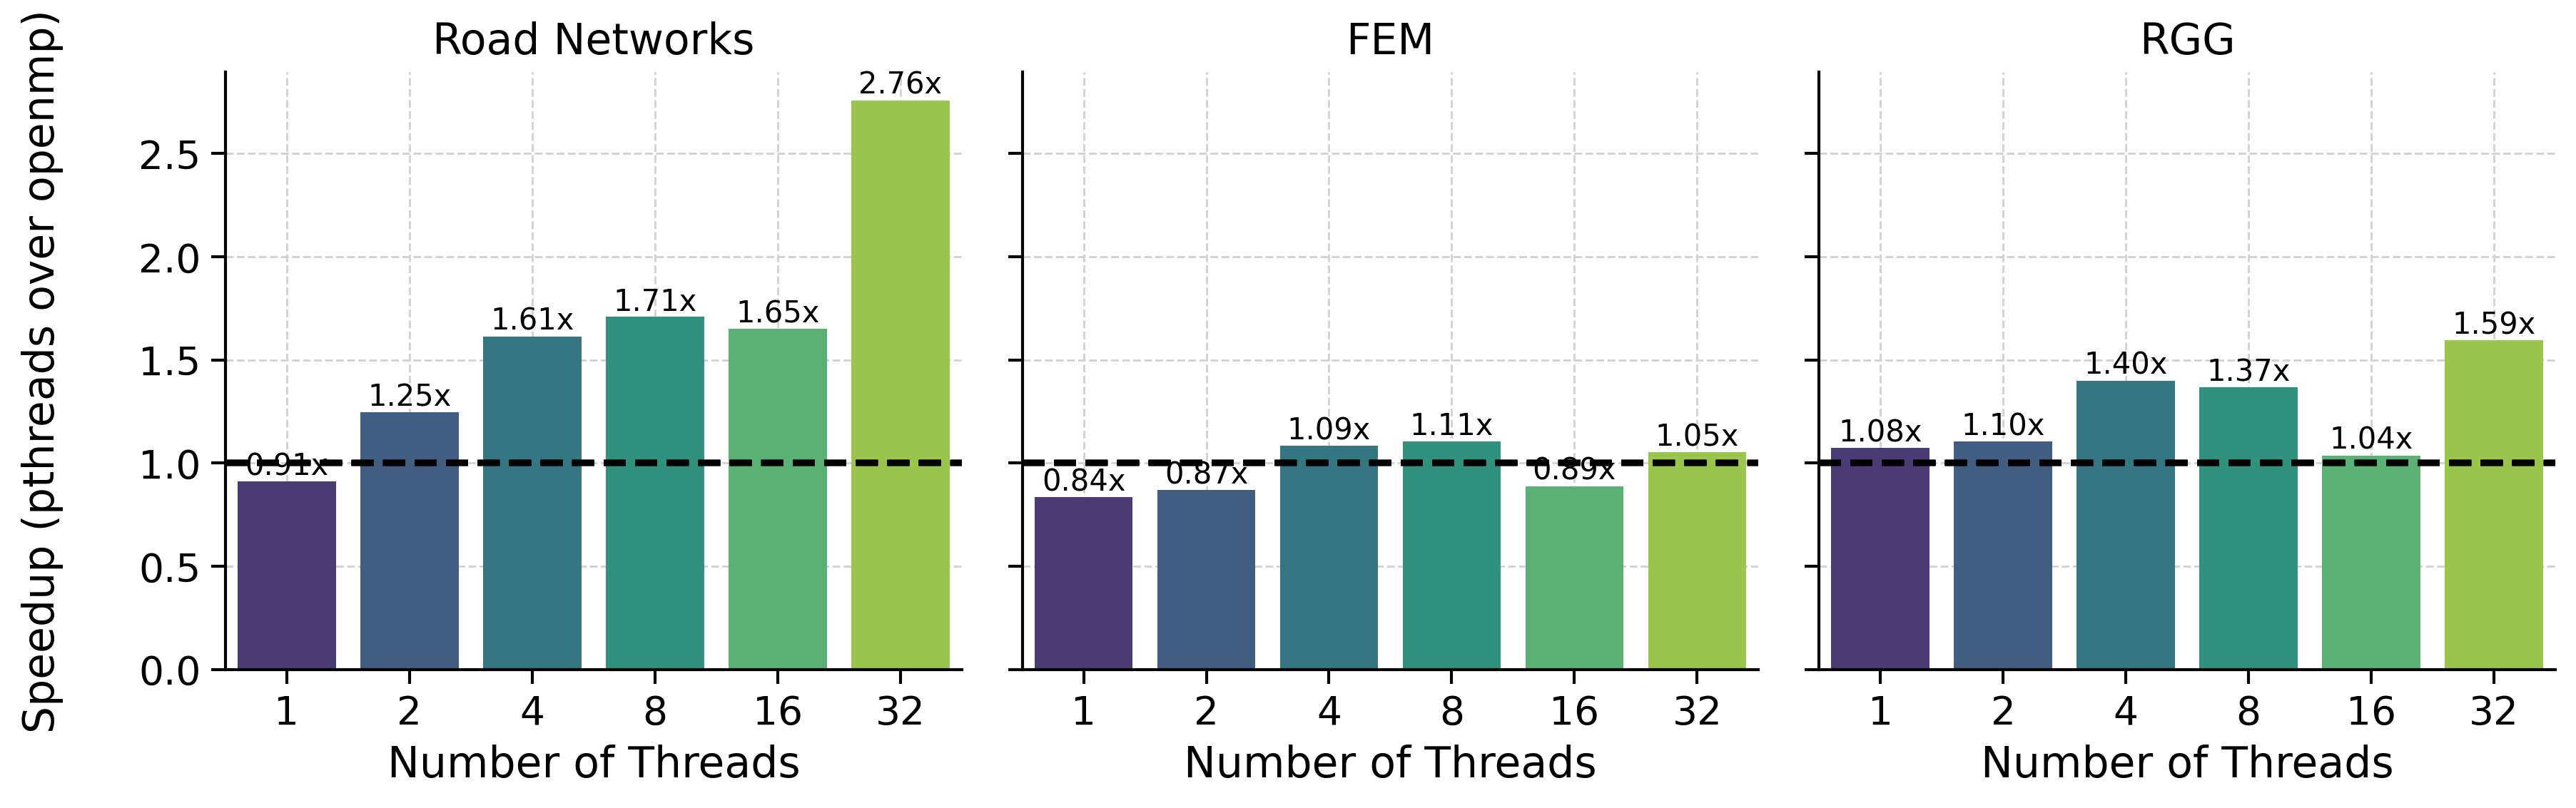
\includegraphics[width=0.7\linewidth]{images/speedup_pthreads.png}
  \vspace{-2mm}
  \caption{\footnotesize Speedup of the pthreads implementation compared to the OpenMP implementation}
\end{figure}
\end{frame}

\begin{frame}{Comparison on different architectures}
\centering
\begin{minipage}{0.8\linewidth}
\begin{figure}
  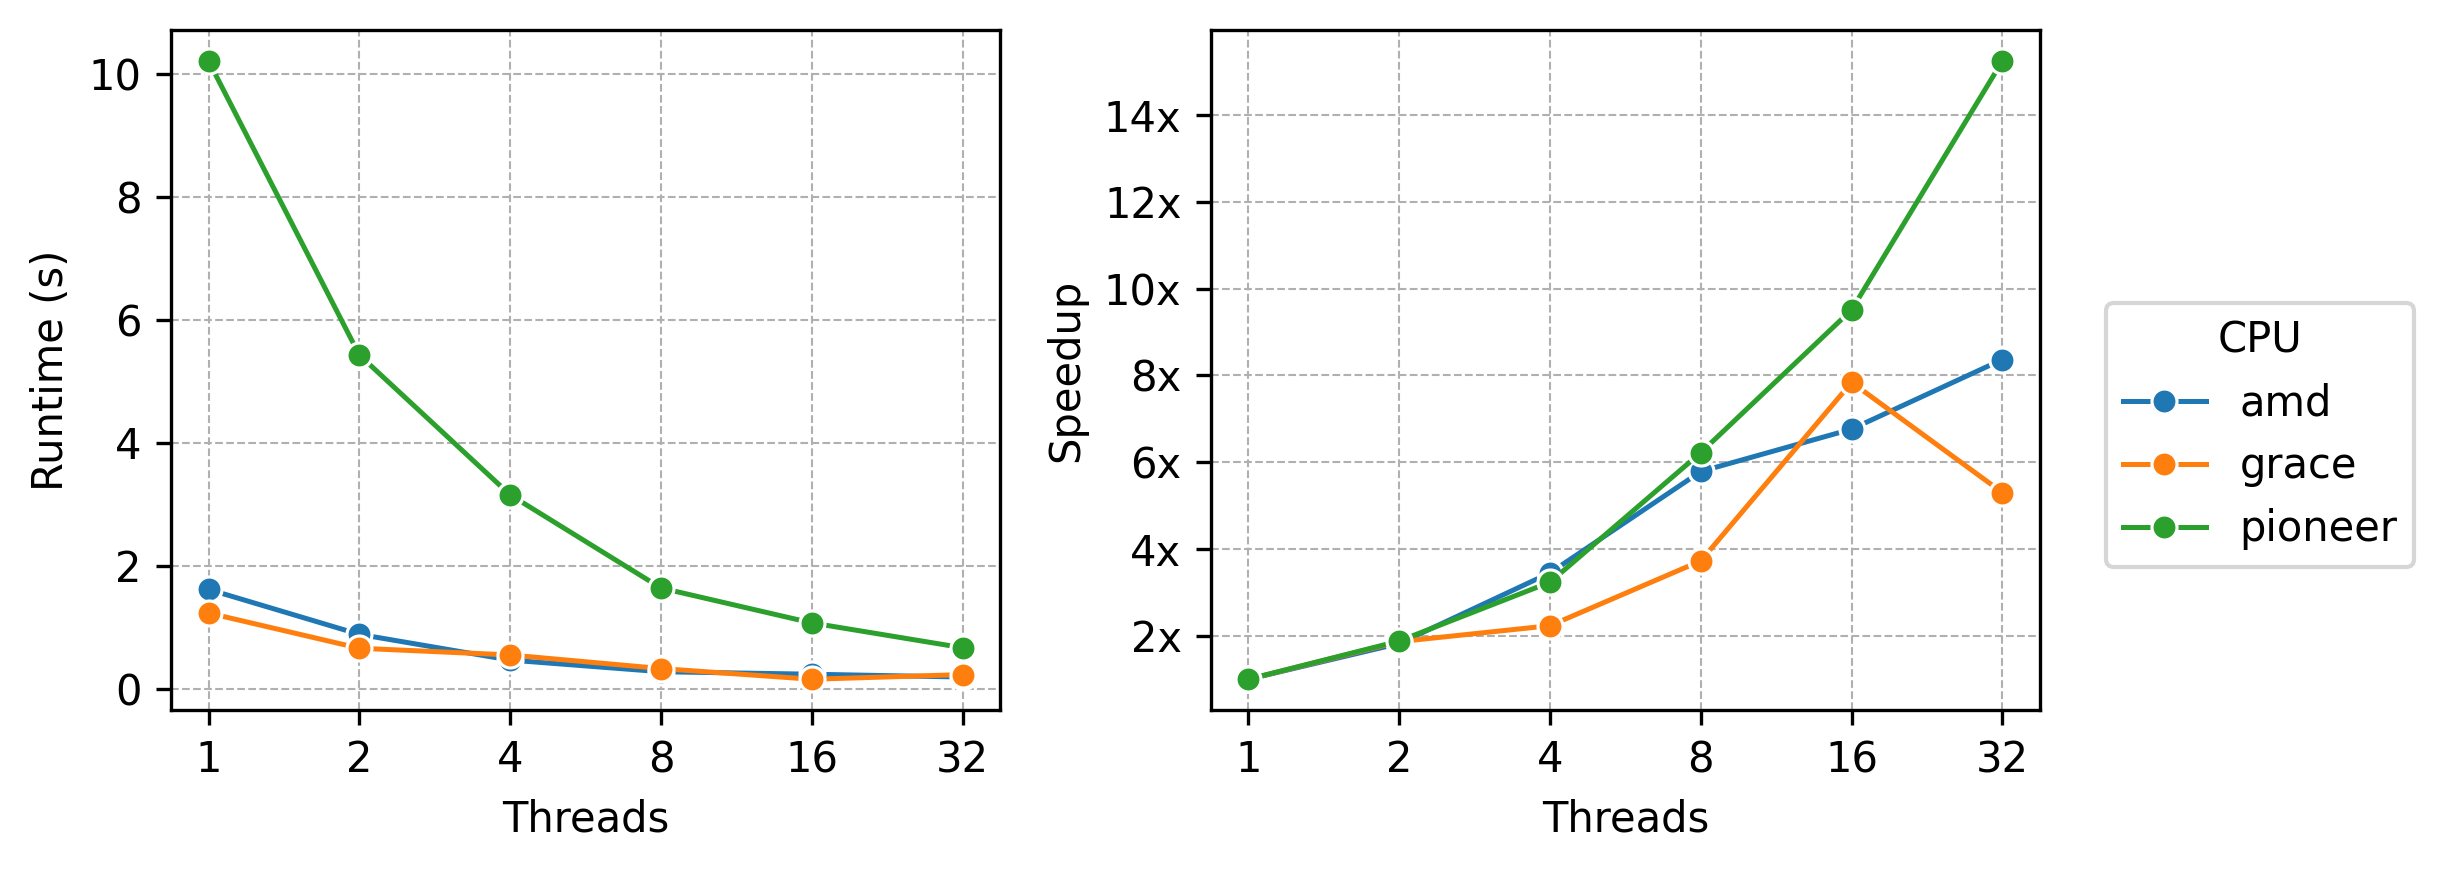
\includegraphics[width=\textwidth]{images/other_platforms.png}
  \caption{\centering Execution time and speedup on different architectures for the Europe road network dataset}
\end{figure}
\end{minipage}
\end{frame}